\chapter{Event Reconstruction
\label{ch:reconstruction}}

Particles created in proton-proton collisions pass through the CMS detector and leave signals in different subdetectors. Figure \ref{fig:cms-slice} shows examples of typical signals for different types of particles. Each type of particle has a different characteristic signature from which it can be identified using information from the various subdetectors. Muons, electrons, and charged hadrons create tracks in the tracker, while photons and neutral hadrons do not. Muons also create hits in the muon systems. Electrons and photons deposit energy in the ECAL, while charged and neutral hadrons deposit most of their energy in the HCAL.

\begin{figure}[hbt]
\begin{center}
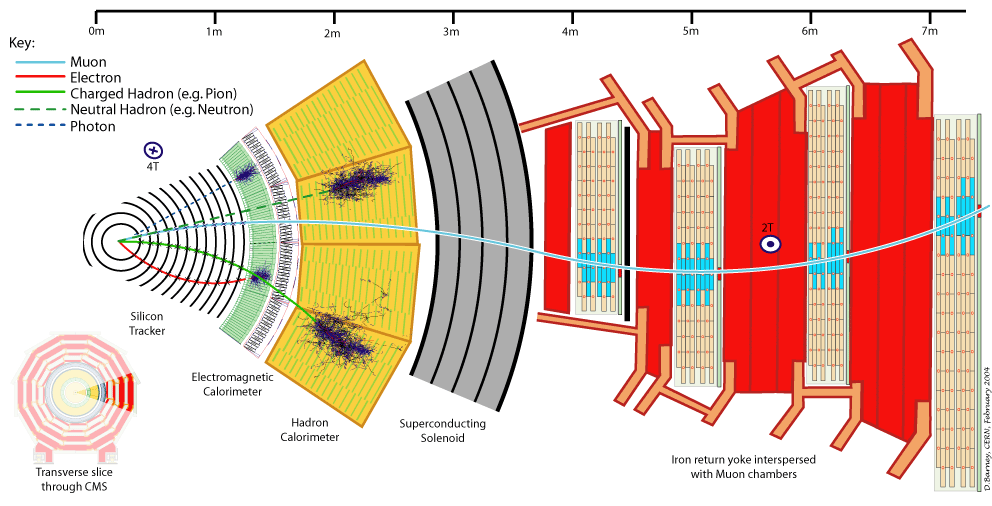
\includegraphics[width=0.95\textwidth]{figures/CMS_slice.png}
\caption{A cross-sectional view of the CMS detector with all subdetectors labeled and examples of signals left by muons, electrons, charged hadrons, neutral hadrons, and photons \cite{CMS-slice}.}
\label{fig:cms-slice}
\end{center}
\end{figure}

The raw output from each subdetector is processed in several steps in order to reconstruct the different types of particles \cite{TDR-software}. The first step is local reconstruction, which involves the creation of reconstructed hits or ``RecHits'' for each subsystem of each subdetector. The tracker RecHits include information about the positions of signals in the form of clusters, which are combinations of contiguous strips or pixels. The muon system RecHits also provide the positions of signals. In the DT and CSC subsystems, these RecHits can be combined into three-dimensional track segments. The ECAL and HCAL RecHits contain the energy, position, and time of energy deposits from traversing particles.

In the second step, global reconstruction, the RecHits from the different subsystems of a given subdetector are combined and further processed. In the tracker, pattern recognition algorithms are employed to reconstruct tracks for various cases, including displaced vertices, low \pt tracks, and high \pt tracks. The ECAL and HCAL RecHits are combined into calorimeter towers or ``CaloTowers'' using a projective $\eta$-$\phi$ geometry. ``Standalone'' muons are created by the muon system global reconstruction, which associates RecHits and track segments in a radial trajectory, accounting for bending by the residual magnetic field, and uses a vertex-constrained fit.

High-level reconstruction is the final step, in which information from all subdetectors is used to reconstruct various types of particles as precisely as possible. The particle types used in this search include electrons, muons, taus, jets, and b-jets. The reconstruction algorithms for these particles will be described in more detail in the following sections of this chapter. Many of these algorithms use particle flow techniques that are unique to CMS and will also be described in more detail.

The CMS experiment uses detailed simulations to predict the performance of the detector and reconstruction algorithms and to model various physics processes. Each simulated event is generated from the interaction of partons in proton-proton collisions and the decays of the resulting particles, based on theoretical calculations. The traversal of the final state particles through the CMS detector is simulated to create simulated hits or ``SimHits''. The effects of photodetectors and readout electronics on these SimHits are also simulated. After that processing, the results can be treated identically to the raw data from real events and used as input for the reconstruction software.

\section{Event Generation}

\section{Detector Simulation}

\section{Particle Flow}

\section{Tracks and Vertices}

\section{Electrons}

\section{Muons}

\section{Taus}

\section{Jets}

\section{b-tagging}